
\chapter{Revisão Bibliografica}

\section{Veculo omnidirecional de 3 rodas}

\section{Roda Omnidirecional}

A roda omnidirecional aparece em vários modelos na literatura, como exemplo o design feito por J. Graboweicki em 1919 \cite{patent_US1305535A}
o design feito por Josef Blumrich em 1972 \cite{patent_US3789947A}.
A roda consiste em rolos perpendiculares (90°) a direção de giro da roda,o efeito é sua capacidade da roda se mover em mais de uma direção ao mesmo tempo.

\begin{figure}[h]
	\centering
	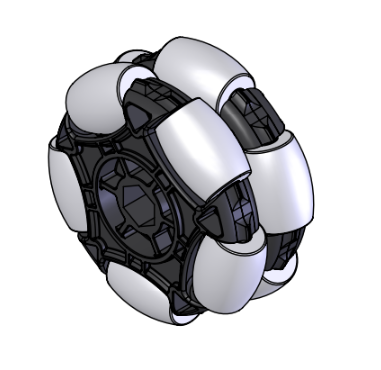
\includegraphics{figures/omniwheel}
	\caption{Modelo de uma Omniwheel \cite{draw_omniwheel}}
\end{figure}

Uma variação da roda omnidirecional é a roda mecanum, inventada por Bengt Ilon \cite{patent_US3876255A}, que possue rolos em 45°.


\section{Microcontrolador STM32F103C8}
O STM32F103C8, também conhecido como Blue Pill, é um microcontrolador fabricado pela STMicroelectronics, de 32-bits, com processador o ARM Cortex-M3, 64Kbs de memória flash.
O processador Cortex-M3, projetado pela ARM (Advanced RISC Machine Ltd.), baseado em arquitetura Harvard, de 32-bits \cite{cortex_m3}.


\begin{figure}[h]
	\centering
	
\includegraphics[width=1.0\textwidth]{figures/stm32f1_pinout}
	\caption{Diagrama de pinos do STM32F103C8}
\end{figure}



\section{Motor DC e drive}


\section{Comunicação serial}


\section{controle PDI}


\section{filtro digital}




